\hypertarget{detector-model-3-level-system}{%
\subsection{Detector model: 3-level
system}\label{detector-model-3-level-system}}

Three-level ``\(\Lambda\)'' system, of interest for * detector models
(decay into a metastable state), * STIRAP * EIT

\begin{lstlisting}[language=Python]
import numpy as np

import matplotlib
import matplotlib.pyplot as plt

from scipy.linalg import expm, norm

# matplotlib.rcParams['text.usetex'] = False

# https://matplotlib.org/gallery/mplot3d/lines3d.html?highlight=parametric
# This import registers the 3D projection, but is otherwise unused.
from mpl_toolkits.mplot3d import Axes3D  # noqa: F401 unused import
\end{lstlisting}

\begin{lstlisting}[language=Python]
matplotlib.rcParams['font.size'] = 14
matplotlib.rcParams['axes.labelsize'] = 16
matplotlib.rcParams['legend.fontsize'] = 16
matplotlib.rcParams['axes.labelpad']  = 14
\end{lstlisting}

\begin{lstlisting}[language=Python]
#matplotlib.rcParams
\end{lstlisting}

\begin{lstlisting}[language=Python]
from IPython.display import display, Latex #, Math
\end{lstlisting}

\begin{lstlisting}
%%javascript
    // do not generate scroll areas, expand figures instead
    IPython.OutputArea.auto_scroll_threshold = 9999
\end{lstlisting}

\begin{lstlisting}
<IPython.core.display.Javascript object>
\end{lstlisting}

\begin{lstlisting}[language=Python]
H = np.array([
    [-2,     0,      32],
    [0,      2,       8],
    [32,     8,       3]
], np.complex_) / 96
\end{lstlisting}

\begin{lstlisting}[language=Python]
def U(t):
    return expm(-1j*H*t)
\end{lstlisting}

\begin{lstlisting}[language=Python]
psi_0 = np.array([1, 0, 0], np.complex_)
\end{lstlisting}

\begin{lstlisting}[language=Python]
def unitary_psi(t):
    return U(t) @ psi_0
\end{lstlisting}

\begin{lstlisting}[language=Python]
def prob(t):
    probabilities = [0, 0, 0]
    for i in 0, 1, 2:
        probabilities[i] = norm(unitary_psi(t)[i])**2
    return probabilities
\end{lstlisting}

\begin{lstlisting}[language=Python]
TMIN, TMAX, TMAX_EXTENDED = 0, 40, 150
TMIN_N, TMAX_N = float(TMIN), float(TMAX)
\end{lstlisting}

\begin{lstlisting}[language=Python]
NPLOTPOINTS = 3200
\end{lstlisting}

\begin{lstlisting}[language=Python]
times = np.linspace(TMIN_N, TMAX_N, num=NPLOTPOINTS)
times_extended = np.linspace(TMIN_N, TMAX_EXTENDED, num=NPLOTPOINTS)
\end{lstlisting}

\begin{lstlisting}[language=Python]
probs = [None, None, None]
for i in 0, 1, 2:
    probs[i] = np.fromiter((prob(t)[i] for t in times), np.float)
#     fig, ax = plt.subplots(figsize=(12, 6*np.max(probs[i])))
#     ax.plot(times, probs[i])
#     plt.show()
\end{lstlisting}

\begin{lstlisting}[language=Python]
# Avoid *tiny* negative numbers, just out of numeric approximation, which will cause problems later,
# when their value is in fact just zero.
probs = np.round(probs, decimals=12)
\end{lstlisting}

\begin{lstlisting}[language=Python]
UNISYM = {
    'psi': u'\u03C8',
    '^2' : u'\u00B2'
}
PROB_LABELS        = ['', '', '']
PROB_AMP_LABELS    = ['', '', '']
PROB_AMP_LABELS_PW = ['', '', '']

for i in 0, 1, 2:
    PROB_AMP_LABELS[i] = '<' + str(i) + '|' + UNISYM['psi'] + '(t)' + '>'
    PROB_LABELS[i]     = '|' + PROB_AMP_LABELS[i] + '|' + UNISYM['^2']

    PROB_AMP_LABELS_PW[i] = '<t|\u2297<%d|\u03A8>>' % i
\end{lstlisting}

https://matplotlib.org/gallery/lines\_bars\_and\_markers/stackplot\_demo.html\#sphx-glr-gallery-lines-bars-and-markers-stackplot-demo-py

\begin{lstlisting}[language=Python]
prob_stack = np.vstack(probs)
\end{lstlisting}

\begin{lstlisting}[language=Python]
colors  =  ['#d44', '#4d4', '#44d']
colors  =  ['r', 'g', 'b']
hatches =  ['\\\\\\', '////////', '...']

linewidths =  [1, 1, 1]

labels     =  PROB_LABELS

fig, ax = plt.subplots(figsize=(12, 6))

stacks = ax.stackplot(times, (probs[0], probs[1], probs[2]))
ax.set_xlabel('t')

for stack, hatch, color, label, linewidth in zip(stacks, hatches, colors, labels, linewidths):
    stack.set_facecolor('w')
    stack.set_edgecolor(color)
    stack.set_label(label)
    stack.set_hatch(hatch)
    stack.set_linewidth(linewidth)

ax.plot(times, probs[0] + probs[1] + probs[2], c='m', label='||\u03C8(t)||\u00B2', linewidth=1.5)

desired_order   = [0, 3, 2, 1]
_handles, _labels = ax.get_legend_handles_labels()
handles         = [ _handles[i] for i in desired_order ]
labels          = [ _labels[i]  for i in desired_order ]
ax.legend(handles, labels, loc='center right', framealpha=1)

plt.savefig('_img/detect3.021/hermitian3color.pdf', bbox_inches='tight', pad_inches=0)
plt.show()
\end{lstlisting}

\begin{figure}[h!]
\centering
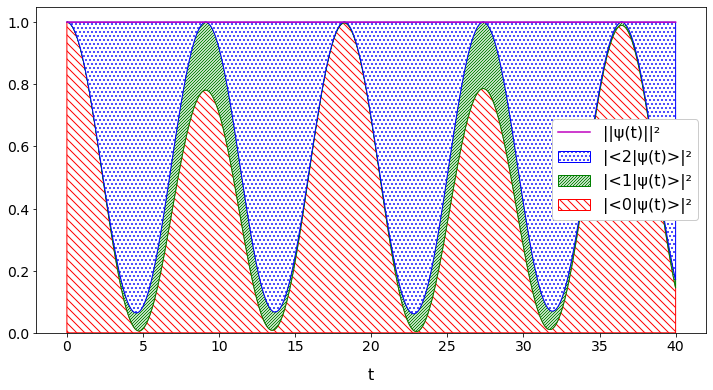
\includegraphics[width=0.66\linewidth]{tex/appendix/nb/jupyter/3lev/output_20_0.png}

\end{figure}

\begin{lstlisting}[language=Python]
rgbs = []
for i in range(NPLOTPOINTS):
    rgbs.append(
        (
            probs[0][i],
            probs[1][i],
            probs[2][i]
        )
    )
\end{lstlisting}

\begin{lstlisting}[language=Python]
fig, ax = plt.subplots(figsize=(12,6))
ax.set_xlabel('t')
ax.scatter(times, np.zeros(NPLOTPOINTS)-0.1,
            c=rgbs, marker='|', s=400)

# "virtual", don't really want to show, only for legend
_c = ['r', '#0a0', 'b']
for i in 0, 1, 2:
    ax.plot(
        times, probs[i],
        c=_c[i],
        linewidth=2,
    )

ax.legend(
    PROB_LABELS,
    loc='upper right'
)

plt.savefig('_img/detect3.021/hermitian3lines.pdf', bbox_inches='tight', pad_inches=0)
\end{lstlisting}

\begin{figure}[h!]
\centering
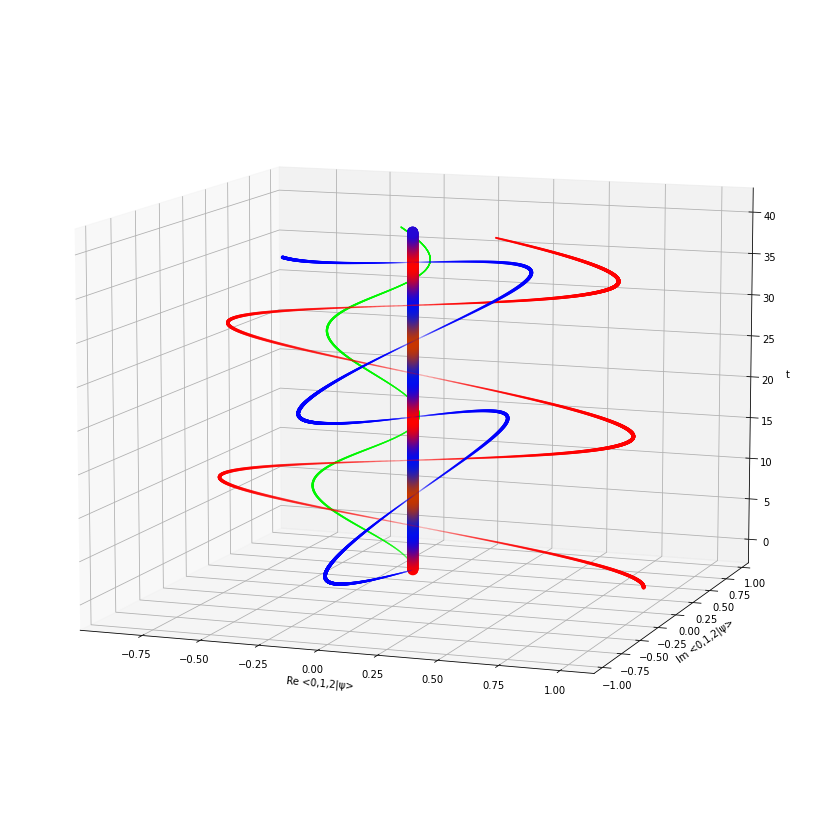
\includegraphics[width=0.66\linewidth]{tex/appendix/nb/jupyter/3lev/output_22_0.png}

\end{figure}

\begin{lstlisting}[language=Python]
unitary_psis = [np.zeros(NPLOTPOINTS)] * 3
for i in 0, 1, 2:
    unitary_psis[i] = np.fromiter( (unitary_psi(t)[i] for t in times), np.complex )
\end{lstlisting}


\begin{lstlisting}[language=Python]
# 3D parametric plot
for (vertical_angle,horizontal_angle,height,width,lloc,view) in (10,-70,12,12,'center left','side'), (80,-120,12,12,'right','top'):
    # fig = plt.figure(figsize=(w5dth, height), dpi=250)2
    fig = plt.figure(figsize=(width, height))

    ax = fig.gca(projection='3d')

    ax.view_init(vertical_angle, horizontal_angle) # rotate 3d point of view

    ax.set_xlabel('Re <0,1,2|\u03C8>')
    ax.set_ylabel('Im <0,1,2|\u03C8>')
    ax.set_zlabel('t')

    ax.scatter(
        np.zeros(NPLOTPOINTS, dtype=np.float),
        np.zeros(NPLOTPOINTS, dtype=np.float),
        times,
        c = rgbs,
        s = 24
    )
    for i in 0, 1, 2:
        ax.plot(
            np.real(unitary_psis[i]),
            np.imag(unitary_psis[i]),
            times,
            label = PROB_AMP_LABELS[i],
            #depthshade=False,
            c = _c[i]
        )
        ax.legend(loc=lloc)
    plt.savefig('_img/detect3.021/hermitianSpaceTime_%s.pdf' % view, bbox_inches=0, pad_inches=0)
\end{lstlisting}

\begin{figure}[h!]
\centering
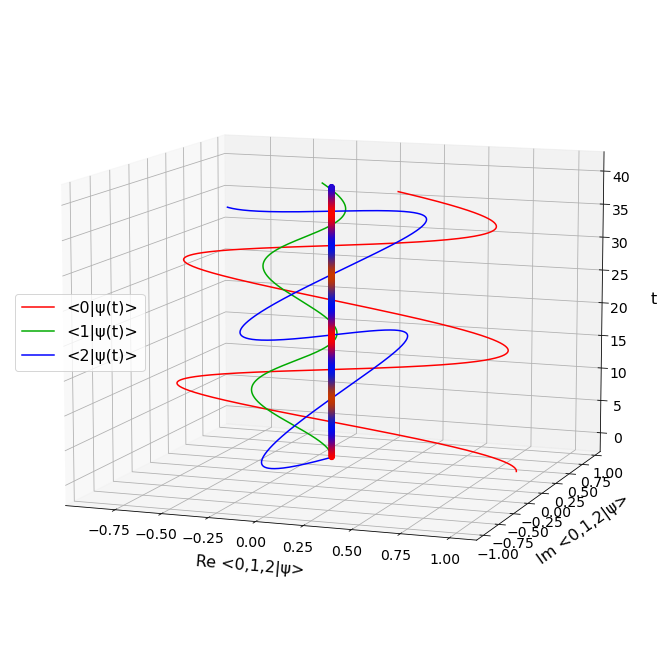
\includegraphics[width=0.66\linewidth]{tex/appendix/nb/jupyter/3lev/output_25_0.png}

\end{figure}

\begin{figure}[h!]
\centering
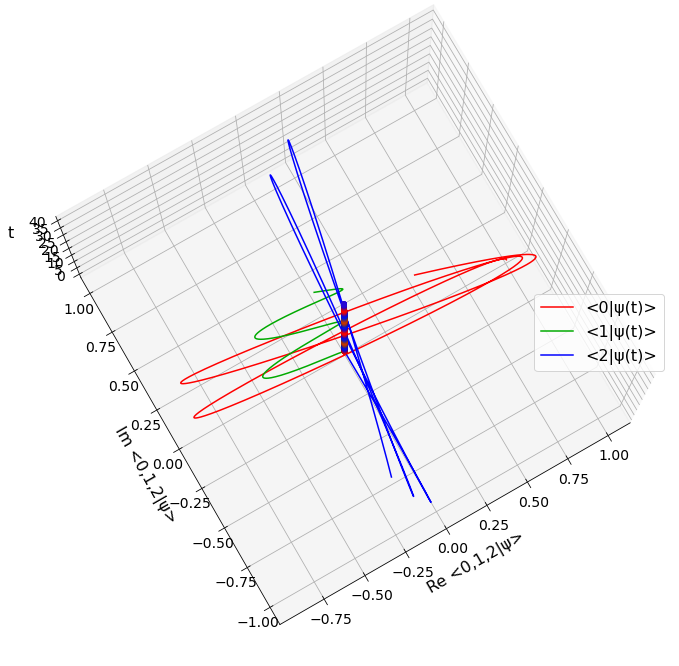
\includegraphics[width=0.66\linewidth]{tex/appendix/nb/jupyter/3lev/output_25_1.png}

\end{figure}

\hypertarget{complex-potential-detection-by-absorption}{%
\subsection{Complex potential (detection by
absorption)}\label{complex-potential-detection-by-absorption}}

\begin{lstlisting}[language=Python]
H_n = H
\end{lstlisting}

\begin{lstlisting}[language=Python]
GAMMA = 0.1
\end{lstlisting}

\begin{lstlisting}[language=Python]
def D(_gamma=GAMMA):
    # no 1/2 factor, absorbed in the _gamma in the matrix here
    return np.array([
        [0, 0,      0],
        [0, 0,      0],
        [0, 0, _gamma]
    ], dtype=np.complex)
\end{lstlisting}

\begin{lstlisting}[language=Python]
D()
\end{lstlisting}

\begin{lstlisting}
array([[0. +0.j, 0. +0.j, 0. +0.j],
       [0. +0.j, 0. +0.j, 0. +0.j],
       [0. +0.j, 0. +0.j, 0.1+0.j]])
\end{lstlisting}

\begin{lstlisting}[language=Python]
def K(_gamma=GAMMA):
    return H_n - 1j*D(_gamma)
\end{lstlisting}

\begin{lstlisting}[language=Python]
K()
\end{lstlisting}

\begin{lstlisting}
array([[-0.02083333+0.j ,  0.        +0.j ,  0.33333333+0.j ],
       [ 0.        +0.j ,  0.02083333+0.j ,  0.08333333+0.j ],
       [ 0.33333333+0.j ,  0.08333333+0.j ,  0.03125   -0.1j]])
\end{lstlisting}

\begin{lstlisting}[language=Python]
def B(_t, _gamma=GAMMA):
    return expm(-1j*K(_gamma)*_t)
\end{lstlisting}

\begin{lstlisting}[language=Python]
B(0)
\end{lstlisting}

\begin{lstlisting}
array([[1.+0.j, 0.+0.j, 0.+0.j],
       [0.+0.j, 1.+0.j, 0.+0.j],
       [0.+0.j, 0.+0.j, 1.+0.j]])
\end{lstlisting}

\begin{lstlisting}[language=Python]
def non_unitary_psi(_t, _gamma=GAMMA):
    return B(_t, _gamma) @ psi_0
\end{lstlisting}

\begin{lstlisting}[language=Python]
evolution = np.zeros((3, NPLOTPOINTS), dtype=np.complex)
evolution_extended = np.zeros((3, NPLOTPOINTS), dtype=np.complex)

for i in 0, 1, 2:
    _iter = (non_unitary_psi(_t)[i] for _t in times)
    _iter_extended = (non_unitary_psi(_t)[i] for _t in times_extended)

    evolution[i] = np.fromiter(_iter, np.complex)
    evolution_extended[i] = np.fromiter(_iter_extended, np.complex)

_iter_norm = (norm(non_unitary_psi(_t)) for _t in times)
norms = np.fromiter(_iter_norm, np.float)

_iter_norm_extended = (norm(non_unitary_psi(_t)) for _t in times_extended)
norms_extended = np.fromiter(_iter_norm_extended, np.float)
\end{lstlisting}

\begin{lstlisting}[language=Python]
colors  =  ['#f66', '#6d6', '#88f']
colors  =  ['r', 'g', 'b']
hatches =  ['\\\\\\', '////////', '...']
labels     =  PROB_LABELS

fig, ax = plt.subplots(figsize=(12, 8))

ax.plot(times, np.ones(NPLOTPOINTS), c='grey', linestyle='dashed', label='Initial norm', linewidth=2.5)

ax.plot(times, norms**2, c='m', linewidth=1.5, label='||\u03C8(t)||\u00B2')

stacks = ax.stackplot(times, (
    np.abs(evolution[0])**2,
    np.abs(evolution[1])**2,
    np.abs(evolution[2])**2
))

ax.set_xlabel('t')

for stack, hatch, color, label in zip(stacks, hatches, colors, labels):
    stack.set_linewidth(.5)
    stack.set_facecolor('w')
    stack.set_edgecolor(color)
    stack.set_label(label)
    stack.set_hatch(hatch)

handles, labels = ax.get_legend_handles_labels()
desired_order = [0, 1, 4, 3, 2]
handles = [ handles[i] for i in desired_order ]
labels  = [  labels[i] for i in desired_order ]
ax.legend(handles, labels, loc='center')

plt.savefig('_img/detect3.021/loss3color.pdf', bbox_inches='tight', pad_inches=0)
plt.show()
\end{lstlisting}

\begin{figure}[h!]
\centering
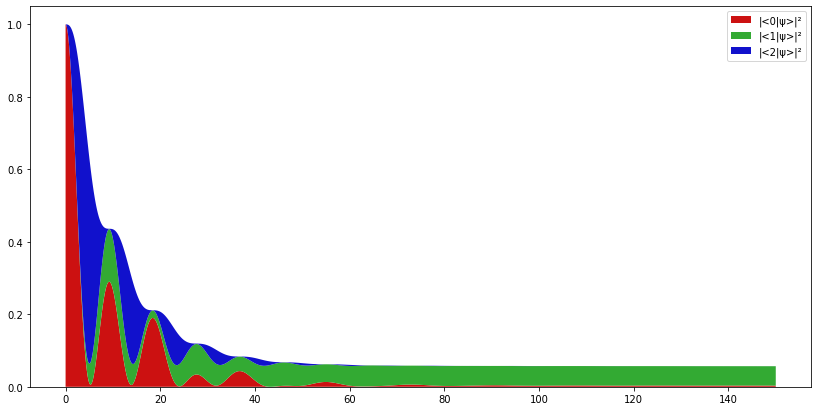
\includegraphics[width=0.66\linewidth]{tex/appendix/nb/jupyter/3lev/output_37_0.png}

\end{figure}

\begin{lstlisting}[language=Python]
# loss of normalization, or integral of antiderivative...
bayesian_denominator_nonpw = 1 - norm(evolution.T[NPLOTPOINTS-1])**2  # TODO! explain/replace
\end{lstlisting}

\begin{lstlisting}[language=Python]
fig, ax = plt.subplots(figsize=(12, 8))
ax.set_xlabel('t')
ax.set_ylabel('Detection probability density  =  - d||\u03C8(t)||\u00B2 / dt')
ax.plot(times, -np.gradient(norms**2, times), c='y', linewidth=3)
plt.savefig('_img/detect3.021/loss.pdf', bbox_inches='tight', pad_inches=0)
\end{lstlisting}

\begin{figure}[h!]
\centering
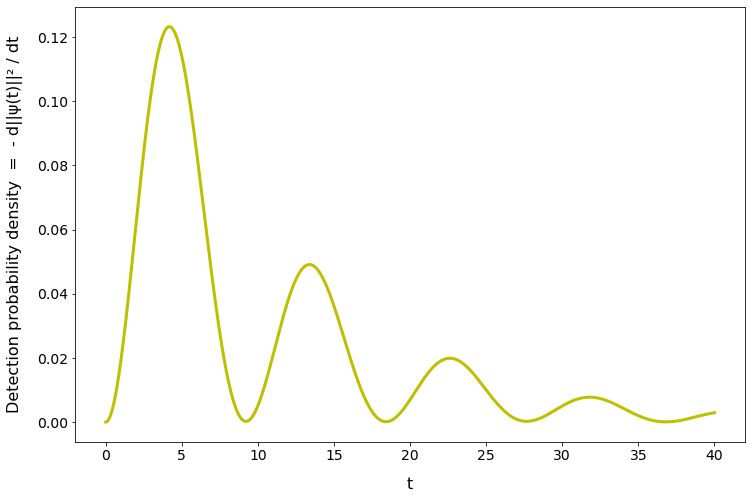
\includegraphics[width=0.66\linewidth]{tex/appendix/nb/jupyter/3lev/output_39_0.png}

\end{figure}

\begin{lstlisting}[language=Python]
labels = PROB_LABELS

colors  =  ['r', 'g', '#ccf']
hatches =  ['\\\\\\\\', '///////', '.....']

fig, ax = plt.subplots(figsize=(14, 7))

ax.set_xlabel('t')

ax.plot(times_extended, np.ones(NPLOTPOINTS), c='grey', linestyle='dashed', label='Initial norm')

ax.plot(times_extended, norms_extended**2, c='m', linewidth=1, label='||\u03C8(t)||\u00B2')

stacks = ax.stackplot(times_extended, (
    np.abs(evolution_extended[0])**2,
    np.abs(evolution_extended[1])**2,
    np.abs(evolution_extended[2])**2
))

for stack, hatch, color, label in zip(stacks, hatches, colors, labels):
    stack.set_linewidth(1.25)
    stack.set_facecolor('w')
    stack.set_edgecolor(color)
    stack.set_label(label)
    stack.set_hatch(hatch)

handles, labels = ax.get_legend_handles_labels()
desired_order = [0, 1, 4, 3, 2]
handles = [ handles[i] for i in desired_order ]
labels  = [  labels[i] for i in desired_order ]
ax.legend(handles, labels, loc='center')

plt.savefig('_img/detect3.021/loss3color_ext.pdf', bbox_inches='tight', pad_inches=0)
plt.show()
\end{lstlisting}

\begin{figure}[h!]
\centering
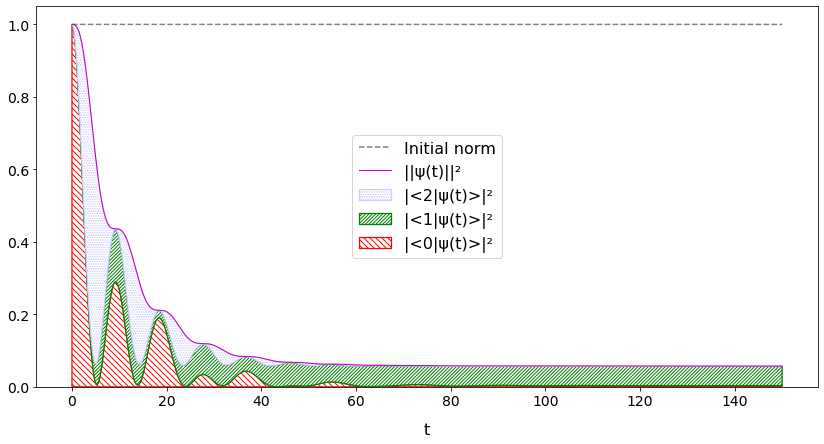
\includegraphics[width=0.66\linewidth]{tex/appendix/nb/jupyter/3lev/output_40_0.png}

\end{figure}

\hypertarget{asymptotic-fidelity-for-1}{%
\subsubsection*{``Asymptotic'' fidelity for $\ket{1}$}\label{asymptotic-fidelity-for-1}}

\begin{lstlisting}[language=Python]
times_extended[-1]
\end{lstlisting}

\begin{lstlisting}
150.0
\end{lstlisting}

\begin{lstlisting}[language=Python]
norms_extended[-1]**2
\end{lstlisting}

\begin{lstlisting}
0.05684539507975811
\end{lstlisting}

\begin{lstlisting}[language=Python]
(np.abs(evolution_extended[1])**2)[-1] / norms_extended[-1]**2
\end{lstlisting}

\begin{lstlisting}
0.9414855990054901
\end{lstlisting}

\hypertarget{detection-probability}{%
\subsubsection{Detection probability}\label{detection-probability}}

\begin{lstlisting}[language=Python]
_detection_prob = -np.gradient(norms_extended**2, times_extended)
fig, ax = plt.subplots(figsize=(14, 7))
ax.set_xlabel('t')
ax.set_ylabel('Detection probability density  =  - d||\u03C8(t)||\u00B2 / dt')
ax.plot(times_extended, _detection_prob, c='y', linewidth=3)
plt.savefig('_img/detect3.021/loss_ext.pdf', bbox_inches='tight', pad_inches=0)
\end{lstlisting}

\begin{figure}[h!]
\centering
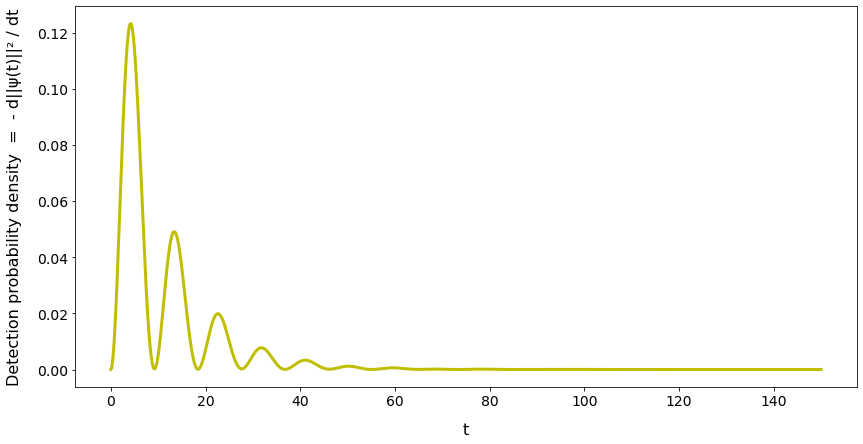
\includegraphics[width=0.66\linewidth]{tex/appendix/nb/jupyter/3lev/output_46_0.png}

\end{figure}

\hypertarget{d}{%
\paragraph{``3D''}\label{d}}

\begin{lstlisting}[language=Python]
# 3D parametric plot

for (vertical_angle,horizontal_angle,height,width,lloc,view) in (15,-80,15,15,'center left','side'), (90, -80, 15, 15,'center left','top'):
    fig = plt.figure(figsize=(width, height))

    ax = fig.gca(projection='3d')

    ax.view_init(vertical_angle, horizontal_angle) # rotate 3d point of view

    ax.set_xlabel('Re <0,1,2|\u03C8>')
    ax.set_ylabel('Im <0,1,2|\u03C8>')
    ax.set_zlabel('t')

    ax.scatter(
        np.zeros(NPLOTPOINTS, dtype=np.float),
        np.zeros(NPLOTPOINTS, dtype=np.float),
        times,

        c = np.array([
            np.abs(evolution[0])**2,
            np.abs(evolution[1])**2,
            np.abs(evolution[2])**2
        ]).T,
        s = 24,
        marker='o'
    )
    _c = ['r', 'g', 'b']

    for i in 0, 1, 2:
        ax.plot(
            np.real(evolution[i]),
            np.imag(evolution[i]),
            times,
            #depthshade=False,
            c = _c[i],
            linewidth=2,
            label = PROB_AMP_LABELS[i]
        )
        ax.legend(loc=lloc)
    plt.savefig('_img/detect3.021/NonHermitianSpaceTime_%s.pdf' % view, bbox_inches='tight', pad_inches=0)
\end{lstlisting}

\begin{figure}[h!]
\centering
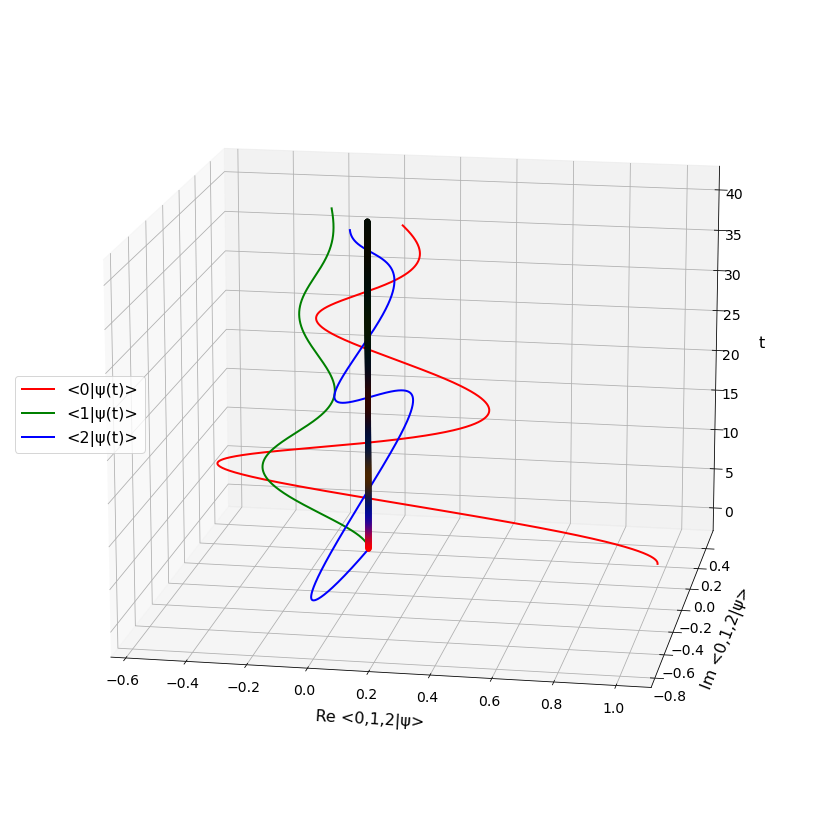
\includegraphics[width=0.66\linewidth]{tex/appendix/nb/jupyter/3lev/output_48_0.png}
\end{figure}

\begin{figure}[h!]
\centering
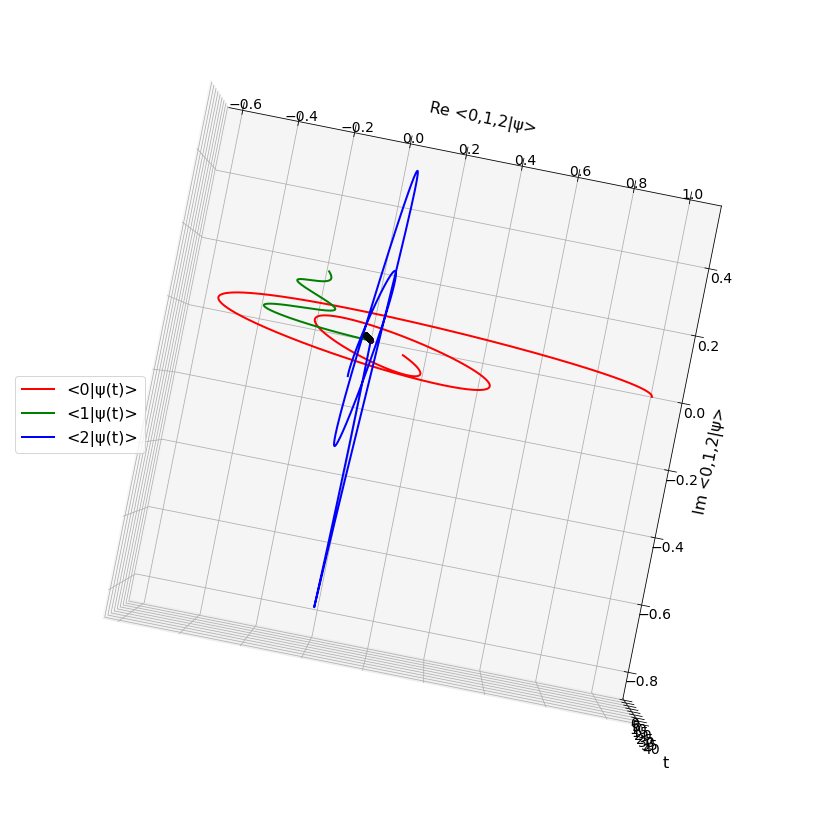
\includegraphics[width=0.66\linewidth]{tex/appendix/nb/jupyter/3lev/output_48_1.png}

\end{figure}

\hypertarget{page-wootters}{%
\subsection{Page-Wootters}\label{appendix:jupyter:3lev:page-wootters}}

\begin{lstlisting}[language=Python]
from scipy.linalg import dft, norm, expm, det, inv
\end{lstlisting}

\begin{lstlisting}[language=Python]
# Dimension of the system, or the spatial/"ordinary" Hilbert space
NS = 3
# Number of levels of the clock aka dimension of Time Hilbert space
NT = 60
# "Period"
DT = TMAX_N  # assume we start with time 0

T = DT * np.diag(np.arange(NT)) / NT
\end{lstlisting}

\begin{lstlisting}[language=Python]
\end{lstlisting}

\begin{lstlisting}[language=Python]
F = dft(NT, scale='sqrtn')
F_dagger = F.conj().T
\end{lstlisting}

\begin{lstlisting}[language=Python]
Omega = F_dagger @ T @ F * 2*np.pi * NT / DT**2
\end{lstlisting}

\begin{lstlisting}[language=Python]
J = np.kron(Omega, np.eye(3)) + np.kron(np.eye(NT), K())
\end{lstlisting}

\begin{lstlisting}[language=Python]
eigenvalues, eigenvectors = np.linalg.eig(J)
\end{lstlisting}

\begin{lstlisting}[language=Python]
eigenvectors = eigenvectors.T
\end{lstlisting}

\begin{lstlisting}[language=Python]
eigenvectors_normalized_in_S = np.empty((NT*NS, NT*NS), dtype=complex)

for i in range(NT*NS):
    eigenvectors_normalized_in_S[i] = eigenvectors[i] / norm(eigenvectors[i][:3])
\end{lstlisting}

\begin{lstlisting}[language=Python]
histories = np.empty((NT*NS, NT*NS), dtype=complex)

for i in range(NT*NS):
    histories[i] = \
        expm(np.kron( -1j*T*eigenvalues[i], np.eye(NS) )) @ \
        eigenvectors_normalized_in_S[i]
\end{lstlisting}

\begin{lstlisting}[language=Python]
# Only implemented for NS=3
def find_linear_independent_initial(eigenvectors=eigenvectors_normalized_in_S):
    best_i, best_j, best_k = -1, -1, -1
    best_det = 0
    best_states = np.array([
        [0, 0, 0],
        [0, 0, 0],
        [0, 0, 0]
    ])
    for i in range(NT*NS):
        for j in range(i, NT*NS):
            for k in range(j, NT*NS):
                # this normalization is not necessary if default
                # eigenvectors=eigenvectors_normalized_in_S
                # is given
                si = eigenvectors[i][:3]
                si = si / norm(si)
                sj = eigenvectors[j][:3]
                sj = sj / norm(sj)
                sk = eigenvectors[k][:3]
                sk = sk / norm(sk)
                states = np.array([
                    si,
                    sj,
                    sk
                ])
                _det = det(states)
                if abs(abs(_det)-1.0) < abs(abs(best_det) - 1.0):
                    best_det = _det
                    best_i, best_j, best_k = i, j, k
                    best_states = states
                if abs(abs(_det)-1.0) == 0:
                    return best_i, best_j, best_k, best_det
        percent = int(100 * (i + 1) / (NT*NS))
        print(
            str(percent) + '% scanned' + "\tabs(best_det) = " + str(abs(best_det)),
            end="\r", flush=True)

    return best_i, best_j, best_k, best_det

\end{lstlisting}

\begin{lstlisting}[language=Python]
best_i, best_j, best_k, best_det = find_linear_independent_initial()
\end{lstlisting}

\begin{lstlisting}
100% scanned    abs(best_det) = 0.9893579012772128
\end{lstlisting}

\begin{lstlisting}[language=Python]
states = np.array([
    histories[best_i][:NS],
    histories[best_j][:NS],
    histories[best_k][:NS]
])
#assert(np.round(abs(det(states)), decimals=2) == 1.0)
# Find what linear combination would bring to the desired initial state psi_0_n
coeffs = inv(states.T) @ psi_0
\end{lstlisting}

\begin{lstlisting}[language=Python]
history = coeffs.dot(np.array([
    histories[best_i],
    histories[best_j],
    histories[best_k]
]))
\end{lstlisting}

\begin{lstlisting}[language=Python]
# 3D parametric plot

times_discrete = np.diag(T)

psi = history.reshape((-1,NS)).T

for (vertical_angle,horizontal_angle,height,width,lloc,view) in ((10,-120,15,25,'center right','side'), (80,-100,15,25,'center right','top')):
    fig = plt.figure(figsize=(width, height))


    ax = fig.gca(projection='3d')

    ax.view_init(vertical_angle, horizontal_angle) # rotate 3d point of view

    ax.set_xlabel('Re <t|\u2297<0,1,2|\u03A8>>')
    ax.set_ylabel('Im <t|\u2297<0,1,2|\u03A8>>')
    ax.set_zlabel('t')

    ax.scatter(
        np.zeros(NT, dtype=np.float),
        np.zeros(NT, dtype=np.float),
        times_discrete,

        c = np.round((abs(psi.T)**2), 8), # rounding, to avoid number instability causing out-of-range rgb vals
        s = 75,
        marker='o'
    )
    _c = ['r', 'g', 'b']

    for i in range(NS):
        ax.scatter(
            np.real(
                psi[i]
            ),
            np.imag(
                psi[i]
            ),
            times_discrete,

            marker = 's',
            #depthshade=False,
            #s = abs(_psi[i]**2)*60,
            s = 60,
            edgecolor = _c[i],
            facecolor = (0, 0, 0, 0),
            linewidth = 1,

            label = PROB_AMP_LABELS_PW[i]
        )
    ax.legend(loc=lloc)
    plt.savefig('_img/detect3.021/PWSpaceTime_%s.pdf' % view, bbox_inches='tight', pad_inches=0)
\end{lstlisting}

\begin{figure}[h!]
\centering
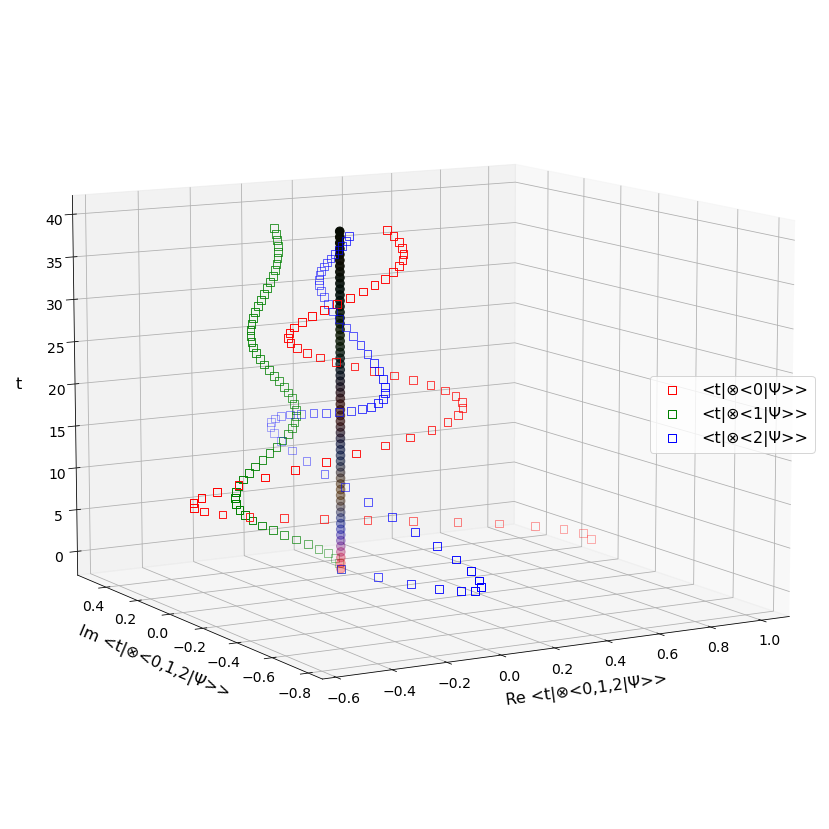
\includegraphics[width=0.66\linewidth]{tex/appendix/nb/jupyter/3lev/output_64_0.png}

\end{figure}

\begin{figure}[h!]
\centering
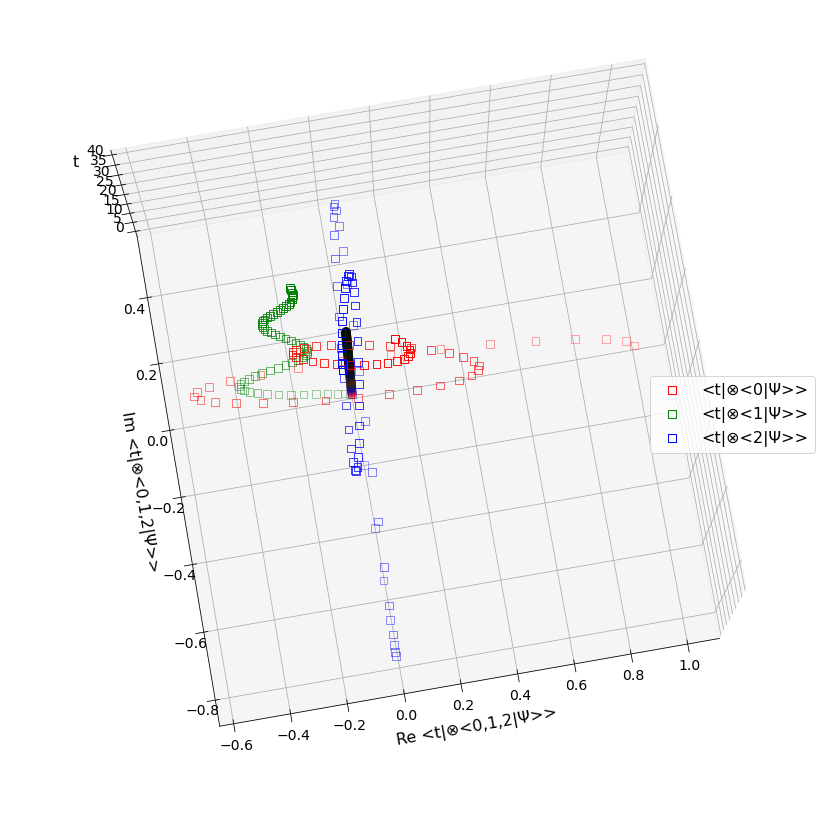
\includegraphics[width=0.66\linewidth]{tex/appendix/nb/jupyter/3lev/output_64_1.png}

\end{figure}

\begin{lstlisting}[language=Python]
norm(psi)**2
\end{lstlisting}

\begin{lstlisting}
18.550562258122728
\end{lstlisting}

\begin{lstlisting}[language=Python]
norm(psi)
\end{lstlisting}

\begin{lstlisting}
4.307036366008851
\end{lstlisting}

\hypertarget{overlapping-pw-and-qm-continuous}{%
\subsubsection{Overlapping PW and QM
continuous}\label{overlapping-pw-and-qm-continuous}}

\begin{lstlisting}[language=Python]
# 3D parametric plot

times_discrete = np.diag(T)

psi = history.reshape((-1,NS)).T

for (vertical_angle,horizontal_angle,height,width,view) in (15,-80,15,15,'side'), (90,-80,15,15,'top'):
    # fig = plt.figure(figsize=(width, height), dpi=300)
    fig = plt.figure(figsize=(width, height))

    ax = fig.gca(projection='3d')

    ax.view_init(vertical_angle, horizontal_angle) # rotate 3d point of view

    ax.set_xlabel('Re')
    ax.set_ylabel('Im')
    ax.set_zlabel('t')

    ax.scatter(
        np.zeros(NT, dtype=np.float),
        np.zeros(NT, dtype=np.float),
        times_discrete,

        c = np.round((abs(psi.T)**2), 8), # rounding, to prevent numeric instability from causing out-of-range RGB values
        s = 75,
        marker='o'
    )
    _c = ['r', 'g', 'b']
    for i in range(NS):
        ax.scatter(
            np.real(
                psi[i]
            ),
            np.imag(
                psi[i]
            ),
            times_discrete,

            marker = 's',
            #depthshade=False,
            #s = abs(_psi[i]**2)*60,
            s = 80,
            edgecolor = _c[i],
            facecolor = (0, 0, 0, 0),
            linewidth = 0.8,
            label = PROB_AMP_LABELS_PW[i]
        )

    # QM continuous
    for i in 0, 1, 2:
        ax.plot(
            np.real(evolution[i]),
            np.imag(evolution[i]),
            times,
            #depthshade=False,
            c = _c[i],
            linewidth=1.5,
            label = PROB_AMP_LABELS[i]
        )
    ax.legend(loc='center left')
    plt.savefig('_img/detect3.021/PWSpaceTimeFit_%s.pdf' % view, bbox_inches='tight', pad_inches=0)
\end{lstlisting}

\begin{figure}[h!]
\centering
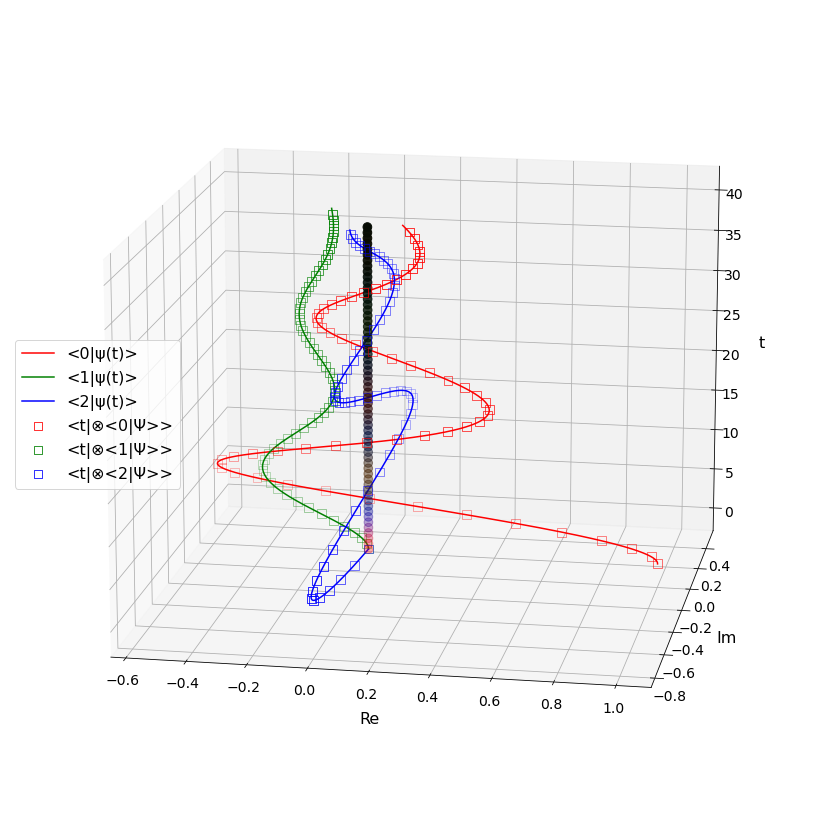
\includegraphics[width=0.66\linewidth]{tex/appendix/nb/jupyter/3lev/output_68_0.png}

\end{figure}

\begin{figure}[h!]
\centering
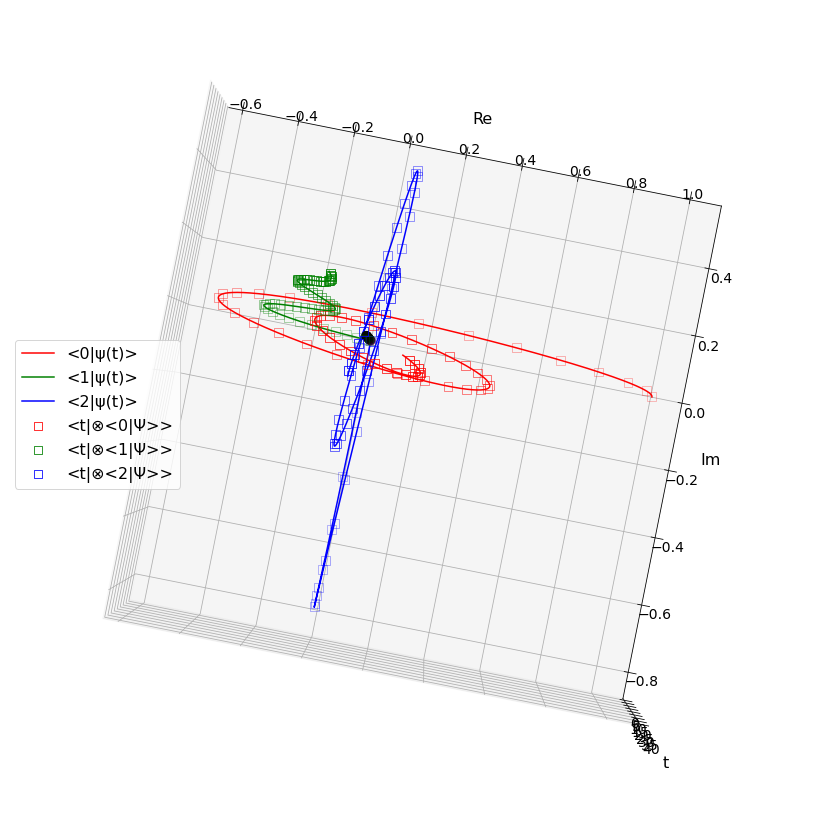
\includegraphics[width=0.66\linewidth]{tex/appendix/nb/jupyter/3lev/output_68_1.png}

\end{figure}

\hypertarget{toa-prob-as-in-macconesacha-arxiv1810.12869}{%
\subsection{TOA prob as in Maccone/Sacha
arXiv:1810.12869}\label{toa-prob-as-in-macconesacha-arxiv1810.12869}}

\emph{Adapted from \(\S\) ``Time of arbitrary event''.}


\begin{lstlisting}[language=Python]
def t_eigenstate(n):
    v = np.zeros(NT, dtype=np.complex)
    v[n] = 1
    return v
\end{lstlisting}

\begin{lstlisting}[language=Python]
arrived_state = np.array([0, 0, 1])
\end{lstlisting}

\begin{lstlisting}[language=Python]
def tn_ox_arrived(n):
    return np.kron(t_eigenstate(n), arrived_state)
\end{lstlisting}

\begin{lstlisting}[language=Python]
history_normalized = history / norm(history)  ## normalized in H_T \otimes H_S
\end{lstlisting}

\begin{lstlisting}[language=Python]
def joint_prob(n):
    return np.abs(tn_ox_arrived(n) @ history_normalized)**2
\end{lstlisting}

\begin{lstlisting}[language=Python]
X = np.arange(NT)

iterable = (joint_prob(n) for n in X)
Y = np.fromiter(iterable, float)
\end{lstlisting}

\begin{lstlisting}[language=Python]
dT  = DT / (NT)
\end{lstlisting}

\begin{lstlisting}[language=Python]
# A "time bin"
X = X * dT # real time
Y = Y / dT # probability _density_
\end{lstlisting}

\begin{lstlisting}[language=Python]
bayes_denominator = np.sum(Y * dT)
Y = Y / bayes_denominator
\end{lstlisting}

\begin{lstlisting}[language=Python]
# fig, ax = plt.subplots(figsize=(12, 8), dpi=300)
fig, ax = plt.subplots(figsize=(12, 8))
ax.set_xlabel('t')
ax.set_ylabel('Detection probability density')
ax.plot(X, Y, 'bs', label='Page-Wootters (Maccone / Sacha -- Bayesian / conditional)')
ax.plot(times, -np.gradient(norms**2, times) / bayesian_denominator_nonpw,
        c='y', linewidth=2, label='Detector model (normalization loss)')
ax.legend()
plt.savefig('_img/detect3.021/conditionalProbFit.pdf', bbox_inches='tight', pad_inches=0)
plt.show()
\end{lstlisting}

\begin{figure}[h!]
\centering
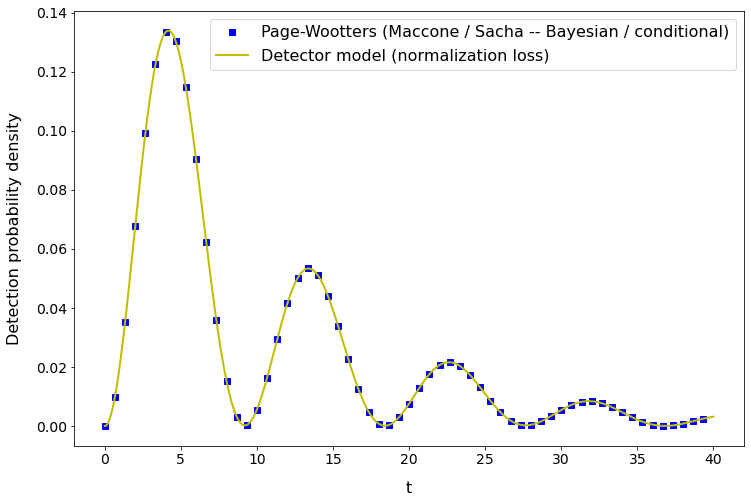
\includegraphics[width=0.66\linewidth]{tex/appendix/nb/jupyter/3lev/output_79_0.png}

\end{figure}

\begin{lstlisting}[language=Python]
nonpw_probs = -np.gradient(norms**2, times) / bayesian_denominator_nonpw
\end{lstlisting}

\begin{lstlisting}[language=Python]
np.sum(nonpw_probs*times[1])
\end{lstlisting}

\begin{lstlisting}
1.0000197507624184
\end{lstlisting}

\begin{lstlisting}[language=Python]
np.sum(Y*dT)
\end{lstlisting}

\begin{lstlisting}
1.0
\end{lstlisting}

\begin{lstlisting}[language=Python]
\end{lstlisting}
